\documentclass[a4paper]{jpconf}
\usepackage{graphicx}
\begin{document}
\title{PyFAI, a versatile library for azimuthal regrouping}

\author{J\'er\^ome Kieffer, Dimitris Karkoulis}

\address{European Synchrotron Radiation Facility; 6 rue Jules Horowitz;
38043 Grenoble; France}

\ead{jerome.kieffer@esrf.fr}

\begin{abstract}
Area ($2d$-) detector like \textsc{ccd} or pixel detectors have replaced
punctual detector over the 15 last years in diffraction (both in \textsc{waxs}, \textsc{saxs} and single crystal
diffraction). Those detectors with wide sensitive area have micron-sized spatial
resolution and provide millions of pixels. PyFAI was designed to reduce \textsc{saxs} and
\textsc{waxs} images taken with those detectors into $1d$ curve (azimuthal integration)
or $2d$ images (transformation named caking), usable by other software like Rietveld
refinement tools.

As a library, the aim of pyFAI is to be integrated in other tools like
PyMca\cite{pymca} or \textsc{edna}\cite{edna} with a clear pythonic interface. But pyFAI
offers also command line tools for batch processing, exporting data in q-space (for \textsc{saxs}) or 2$\theta$ for
(\textsc{waxs}) and a calibration GUI for optimizing the geometry of the setup starting
from  reference sample's \textit{powder rings}.  PyFAI shares the geometry of
\textsc{spd}\cite{spd} but can directly import geometries determined by
\textsc{fit2d}\cite{fit2d1996}.
PyFAI has been designed to work with any kind of detector and geometry (transmission or reflection) and
relies on fabio\cite{fabio}; a library able to read more than 20 image formats
produces by  detectors from 12 different manufacturers.

Even if the basic idea is interpolation from cartesian space $(x,y)$ to polar
space $(2\theta, \chi )$, intensities should be conserved (both local and total)
to get quantitative results.  Those technical details on how integration is implemented
and how it was ported to native C-code and parallelized on graphic card are
discussed  in this paper.
\end{abstract}

\section{Introduction}

With the advent of hyperspectral experiments like diffraction tomography in the
world of synchrotron radiation, existing tools for azimuthal integration like
\textsc{fit2d}\cite{fit2d1996} and \textsc{spd}\cite{spd} reached their limits with the fast data rate
needed by such experiments. Even when integrated into massively parallel
frameworks like \textsc{edna}\cite{edna}, such stand-alone programs, due to their
monolithic nature, could not keep pace with the data flow of new detectors.

\section{Fast azimuthal integration}
This highlights the need for a new tool for performing azimuthal integration
much faster than before, without compromising quality. This tool is
implemented in Python, which is already very popular for data
analysis (PyMca\cite{pymca}, PyNX\cite{pynx}, \ldots) and open source.

\subsection{PyFAI executables}
PyFAI was designed to be used by scientists needing a simple tool for azimuthal
integration. Two command line programs \textit{pyFAI-waxs} and
\textit{pyFAI-saxs} are provided with pyFAI for performing the
integration of one or many images. The \textsc{waxs} version outputs results in
$2\theta /I$  whereas the \textsc{saxs} version outputs $q/I(/\sigma )$.
Options for those programs are parameter files describing the geometry and mask file. They can
also do some  pre-processing like dark-noise subtraction and flat-field correction.

\subsection{A Python library}
PyFAI is first and foremost a library: a tool of the scientific
toolbox built around ipython\cite{ipython} and numpy\cite{numpy} to 
perform data-analysis either interactivly or in scripts.
Figure \ref{notebook} shows an interactive session where an integrator is
created, and image loaded and integrated before being plotted.

\begin{figure}[h]
\begin{center}
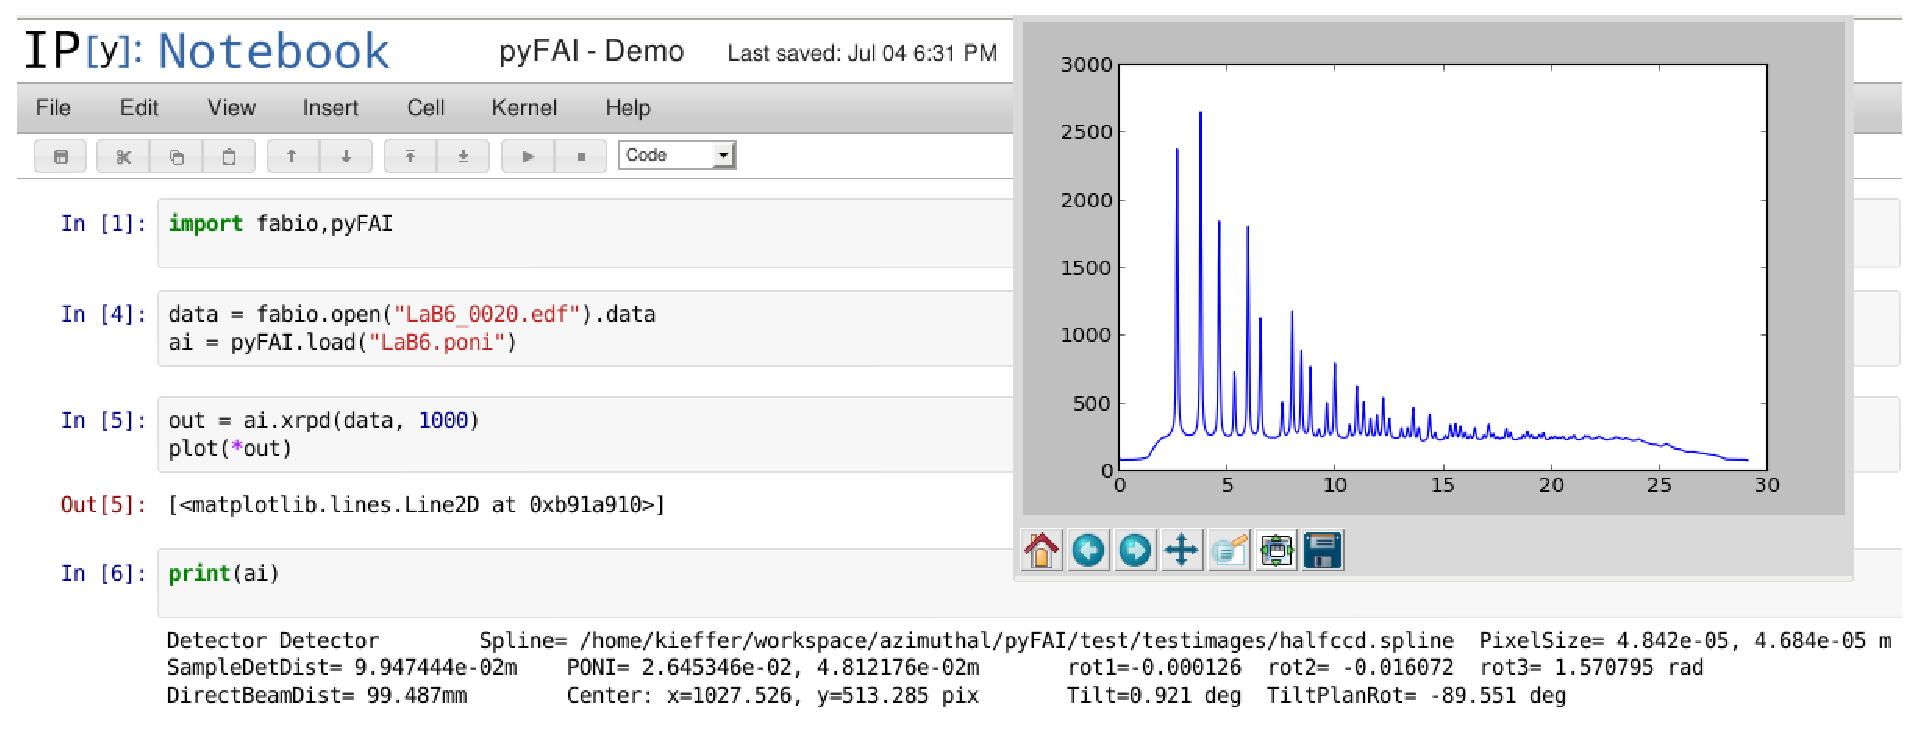
\includegraphics[width=15cm]{img/notebook-l.eps}
\caption{\label{notebook} Example of interactive use of fabio and pyFAI in the
interactive environment ipython.}
\end{center}
\end{figure}

\section{Regrouping mechanism}
Azimuthal-regrouping is done in pyFAI using a histogram-like algorithm: every
pixel of the image is associated to it's coordinate in polar coordinate
$(2\theta , \chi )$ or $(q, \chi )$. Then a couple of histograms of $2\theta$
(or $q$) are build:
one non weighted for measuring the number of pixels falling in each bin and
another weighted by pixel intensities.
The division of the weighted histogram by the number of pixels per bin gives
the powder pattern.
$2d$ regrouping (called \textit{caking} in \textsc{fit2d}) is obtained in the
same way using two-dimensional histograms over radial ($2\theta$ or $q$) and azimuthal angles
($\chi$).

\subsection{Pixel splitting algorithm}
Powder diffraction patterns obtained by histogram have a major weakness where
statistic is low.
%: a high level of  noise is observed close to the beam stop.
This is particularly striking when considering  $2d$-regrouped where most of
the bins close to the beam-stop are not populated by any pixel.
In Figure \ref{rough} many pixels are missing in the low $2\theta$ region
what is not acceptable: the  $2d$-regrouping of a smooth image should be smooth
(Figure \ref{smooth}.

\begin{figure}[h]
%\begin{center}
\begin{minipage}{8cm}
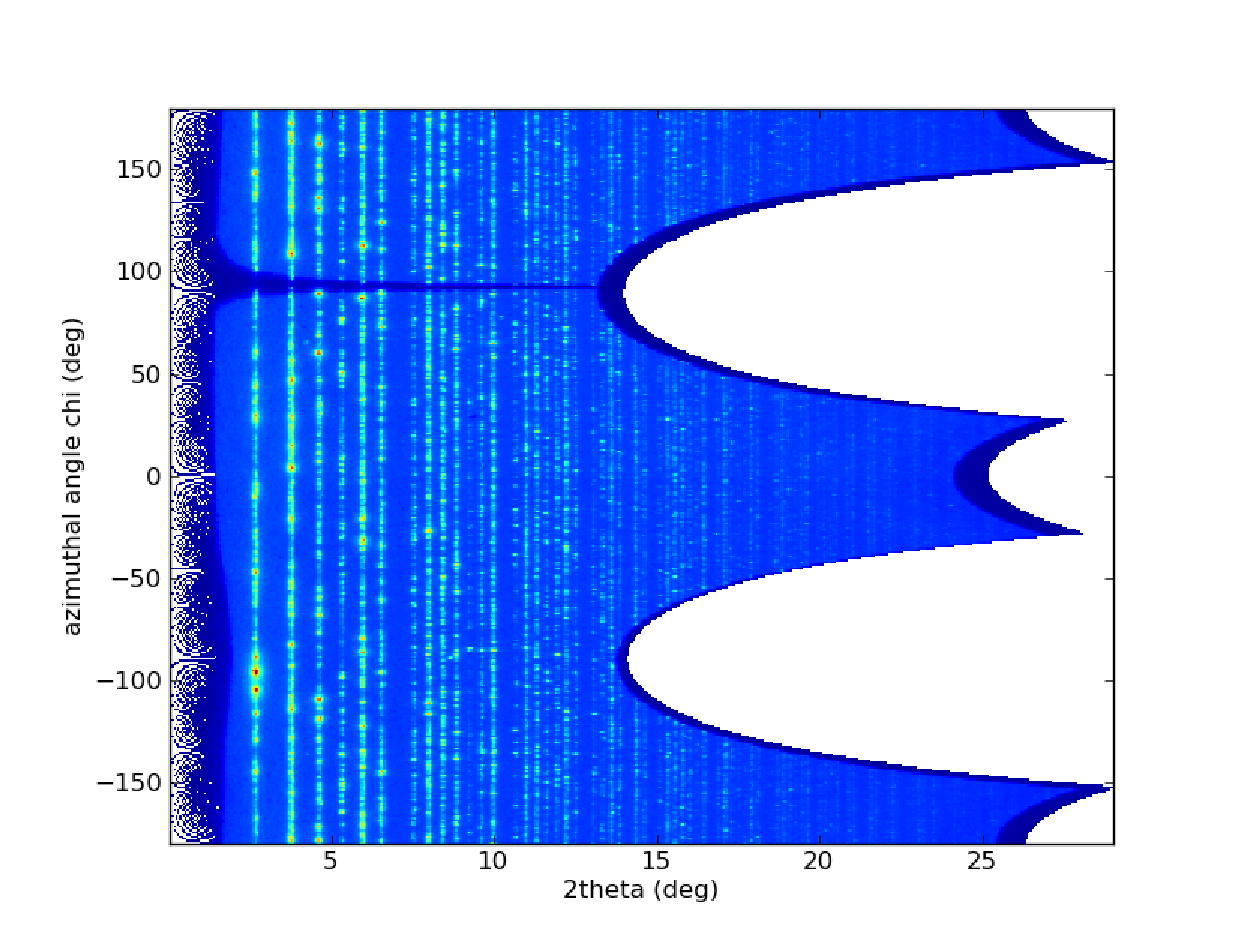
\includegraphics[width=8cm]{img/2Dhistogram.eps}
\caption{\label{rough}$2d$-regrouped image without pixel splitting. Note the
missing pixels near the beam stop and the high-frequency noise patterns.}
\end{minipage}\hspace{5mm}
\begin{minipage}{8cm}
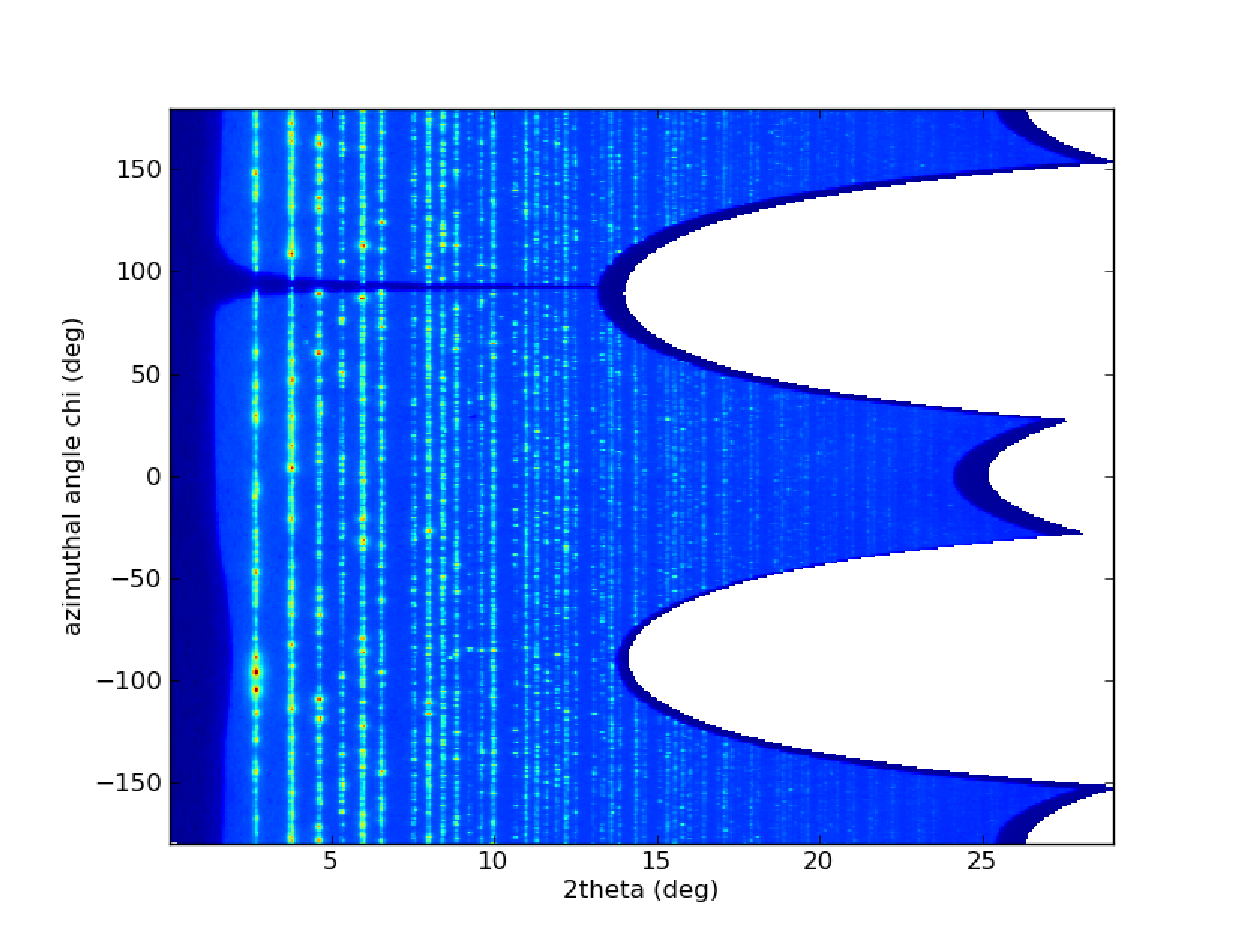
\includegraphics[width=8cm]{img/2DwithSplit.eps}
\caption{\label{smooth}$2d$-regrouped image with pixel splitting. The
transformation of a smooth image remains smooth.}
\end{minipage}
%\end{center}
\end{figure}

PyFAI solves this problem by considering, in addition to the pixel's position,
their spatial extension. Each pixel is then split and distributed over the
corresponding bins; intensity being consdered as homogeneous in a pixel.

\subsection{Performances and migration to native code}
for histograms, computation time is proportional to the size of the input image
and almost independent of the number of bins. Originally the regrouping was implemented
using the histogram provided by numpy\cite{numpy}; then re-implemented in
cython\cite{cython} to achieve a four times speed-up.
The pixel splitting algorithm was also implemented in cython, enhancing the
original histogram and optimized to give excellent single-threaded performances
around 30 Hz.Mpixel.

\subsection{Graphic card implementation}
Graphical Processing Unit (\textsc{gpu}) are composed of hundreds of
small computing cores; they are optimized for highly parallel algorithms
with speed-ups going up to 3 orders of magnitude over sequential code running
on Central Processing Unit (\textsc{cpu}).
While histograms do not fall into this category, they can  nevertheless be
ported to \textsc{gpu} efficiently. In order to benefit from \textsc{gpu} acceleration,
the Open Computing Language\cite{opencl} (OpenCL) was used. OpenCL can make use
of multiple different devices such as \textsc{cpu} and \textsc{gpu} with very 
different features and capabilities.
This framework also allows the code to work on multiple \textsc{cpu} cores, which was
useful for validation. As azimuthal integration is a reduction
of millions of pixels into hundreds of bins, double-precision arithmetics must
be used but it is not available on all OpenCL devices.
Table \ref{perfs} summerizes the execution time for images comming from various
detectors on a dual-processor computer, either using either the single threaded
implementation, either the OpenCL one on the 16 \textsc{cpu} core or the 512
\textsc{gpu} core of the Tesla C2075 or GTX580.

\begin{table}[h]
\begin{center}
\caption{\label{perfs}Performances obtained on a computer with two Intel
Xeon X5690 @3.47GHz and various \textsc{gpu}\\
%: C2075 and GTX580 are professional
%and consumer grade Fermi class nVidia \textsc{gpu} with 512 cores.\\
 The table reports execution time measured in milliseconds on various size of
 images in double precision (except for the AMD FireGL v7800 where single
 precision had to be used).}

\begin{tabular}{|l|c||c|c||c|c|c|c|}
\hline
Image               & Image size 	& \multicolumn{2}{|c||}{\textsc{cpu} X5690}& \multicolumn{4}{|c|}{OpenCL $1d$ regrouping} \\
					& mega pixels	& $1d$	&	$2d$	&	X5690	&	C2075	&	GTX580	&	FireGL* \\
\hline
Pilatus-1M 			& 1  			& 34.4  &	63.1	&	13.9	&	7.2		&	6.3		&	13.8 \\
Half-Frelon 		& 2  			& 76.6  &   132.4   &	23.4	&	14.4	&	12.2	&	18.8 \\
Frelon 				& 4  			& 165.0	&	269.4   &	52.6	&	34.1	&	28.2	&	40.0 \\
Pilatus-6M 			& 6  			& 232.0	&	350.7	&	74.4	&	49.8	&	40.7	&	48.1 \\
Fairchaild 			& 16 			& 613.9	&	849.7   &	158.9	&	99.0	&	96.4	&	95.6 \\
\hline
\end{tabular}
\end{center}
\end{table}

The OpenCL implementation of pyFAI is very fast on \textsc{gpu} offering an extra five
time speed-up over \textsc{cpu} implementation. The profiling of the code revealed new
bottlenecks which will be addressed in future optimisations.

\section{Conclusion}

A library such as pyFAI has two main goals:
\begin{itemize}
\item Performing azimuthal integration witch offers a clean interface to
developers or scientists in the field of X-ray diffraction and provide outstanding performances.
\item No compromise on the quality of the result with a carreful management of
the geometry and precise pixel splitting offerting total and local intensity
conservation.
\end{itemize}

This twenty folds speed up in azimuthal integration opens the door to a new
kind of analysis, not even considered until today: a scientist could write
himself a small script of a dozen of lines of code for analyzing a diffraction
tomography experiment (typically 60 x 200 frames), such analysis would only
take a few minutes using pyFAI when it used to take days for data reduction only.
PyFAI is the tool to couple with the next generation hi-speed detectors.

\subsection*{Acknowledgments}
Authors wish to acknowledge especially Manuel S\'anchez del R\'io for suggesting
the usage of of weighted histograms;
V. Armando Sol\'e for his expertise on developing native code under windows;
Jonathan Wright and all the ESRF-ID11 team for precise specifications validation
and Peter B\"osecke for the geometry setup. Porting pyFAI
to \textsc{gpu} would not have been possible without the financial support of LinkSCEEM-2 (RI-261600).

\subsection*{Appendices}
PyFAI is an open source software released under the GPL licence.
As of July 2012, pyFAI is available in version 0.6 on the EPN-Campus
forge\cite{forge} which includes OpenCL acceleration.
PyFAI depends on Python v2.6 or v2.7, numpy\cite{numpy} and OpenCL\cite{opencl}
In order to be able to read images from various detector, pyFAI relies on the
fabio\cite{fabio} library available from sourceforge. The graphical user
interface for calibration of diffraction setup uses in addition
matplotlib\cite{matplotlib}, scipy\cite{scipy}, and FFTw3\cite{fftw}.
C, C++ compilers and Cython\cite{cython} are needed to build pyFAI from
sources.

PyFAI is packaged and available in common Linux distributions like Debian
7.0 and Ubuntu 12.04. Install packages for Windows are also
available on the EPN-Campus forge.

 \section*{References}
\bibliographystyle{iopart-num}
\bibliography{biblio}

\end{document}


